\chapter{Configuración y ejecución de los entornos de entrenamiento}
\label{cap:configuracion_ejecucion}

% Corregido 08/01/2024
% TODO:daniel: Revisar la configuración y ejecución de los entornos de entrenamiento

En este capítulo se detalla la configuración que se ha realizado para la ejecución de los
del modelo de lenguaje y qué plataformas se han utilizado para la ejecución de los mismos.
En la realización de este proyecto se ha utilizado dos entornos de ejecución diferentes:

\begin{itemize}
    \item \textbf{Entorno local:} se ha utilizado el cluster \textit{sert} del departamento
        de Arquitectura de Computadores de la Universitat Politècnica de Catalunya.
    \item \textbf{Entorno en la nube:} se ha utilizado una plataforma de entrenamiento en la nube
        llamada Lightning IA Studio.
\end{itemize}

\section{Plataforma de desarrollo \textit{lit-gpt}}
\label{sec:lit_gpt}

% Corregido 09/01/2024
% TODO:daniel: Revisar lit-gpt

Lit GPT es una plataforma de desarrollo que nos permite entrenar modelos de
lenguaje de manera sencilla. Esta plataforma nos ofrece una serie de scripts que nos
permiten entrenar modelos utilizando diferentes técnicas de las cuales hemos hablado
en el capítulo \ref{cap:estadoDelArte}. Así mismo, nos ofrece una serie de scripts que nos permiten convertir
los modelos de lenguaje de la plataforma de \textit{huggingface} a un formato que pueda
ser utilizado por el \textit{framework lightning}. Esta plataforma de desarrollo se encuentra
disponible en el siguiente repositorio de GitHub \url{https://github.com/Lightning-AI/lit-gpt.git}.

Algunas de las opciones que son interesantes para este proyecto es que \textit{lit-gpt} nos
permite modificar la precisión de los modelos de lenguaje, es decir, podemos entrenar
modelos de lenguaje con una precisión de 16 bits o de 32 bits. Así mismo, nos permite
aplicar técnicas de cuantización. Estas técnicas de cuantización nos permiten reducir
el tamaño de los modelos de lenguaje y reducir su consumo de memoria.
Para poder aplicar estas técnicas \textit{lit-gpt} nos ofrece una serie de opciones que
podemos pasar a los scripts de entrenamiento. En la tabla \ref{tab:opciones_litgpt} 
tenemos las opciones que nos ofrece \textit{lit-gpt}.

\begin{table}[H]
    \centering
    \resizebox{\textwidth}{!}{%
    \begin{tabular}{|l|l|l|}
    \hline
    \rowcolor[HTML]{8EA9D8} 
    Opción      & Descripción                                                                                                                                                  & Posibles valores                                                                                              \\ \hline
    --precision & \begin{tabular}[c]{@{}l@{}}Define la precisión de los pesos, 16 bits o 32 bits.\\ Esta opción depende mucho de la compatibilidad del\\ hardware\end{tabular} & {[}16-true, bf16-true, 32-true{]}                                                                             \\ \hline
    --quantize  & \begin{tabular}[c]{@{}l@{}}Define el método de cuantificación que se le aplicará\\ al modelo\end{tabular}                                                    & \begin{tabular}[c]{@{}l@{}}{[}bnb.nf4, bnb.nf4-dq, bnb.fp4,\\ bnb.fp4-dq, bnb.int8, gptq.int4{]}\end{tabular} \\ \hline
    \end{tabular}%
    }
    \caption[Opciones que nos ofrece \textit{lit-gpt}]{Opciones que nos ofrece \textit{lit-gpt} (Elaboración propia)}
    \label{tab:opciones_litgpt}
\end{table}

\section{Configuración}
\label{sec:configuracion}

\subsection{Cluster AC: \textit{Sert}}
\label{subsec:cluster_ac}

% Corregido 09/01/2024
% TODO:daniel: Revisar cluster AC

El clúster de AC es un clúster de computación de alto rendimiento que dispone el departamento
de Arquitectura de Computadores de la Universitat Politècnica de Catalunya. Este clúster dispone
de un nodo con GPU's que recibe el nombre de \textit{sert-2001}. Este nodo tiene las siguientes
características técnicas:

\begin{itemize}
    \item 1 nodo 2x Intel Xeon Silver 4210R a 2.40Ghz
    \item 128 GB de memoria RAM
    \item 2 discos duros de 480GB SSD
    \item 2 discos duros de 2TB NVME
    \item 2 tarjetas de red 10 Gigabit Ethernet
    \item 8 GPU NVIDIA RTX 2080TI 11 GB GDDR6 PCIe
\end{itemize}

La conexión con el cluster se realiza a través de una VPN proporcionada por el departamento
de Arquitectura de Computadores. Una vez conectado a la VPN, se puede acceder al cluster
a través de SSH. El cluster dispone de un sistema de colas de ejecución de trabajos. Para
enviar un trabajo a ejecutar en el cluster se utiliza el comando \textit{sbatch}. En la figura
\ref{tab:colaGPU} tenemos la definición de las colas que disponemos para este nodo. Así mismo,
nos podemos conectar de forma interactiva a un nodo del cluster utilizando el comando
\textit{srun}.

\begin{table}[H]
    \centering
    \resizebox{\textwidth}{!}{%
    \begin{tabular}{|l|l|l|l|l|}
    \hline
    \rowcolor[HTML]{8EA9D8} 
    Cola        & Disponibilidad de GPU's & Tiempo maximo de ejecución & Otros limites                                                                                    & Observaciones    \\ \hline
    big\_gpu    & máximo 8, mínimo 5      & 4 horas                    &                                                                                                  &                  \\ \hline
    medium\_gpu & máximo 4, mínimo 2      & 2 dias                     & \begin{tabular}[c]{@{}l@{}}1 trabajo en ejecución\\ mínimo entre todos los usuarios\end{tabular} &                  \\ \hline
    small\_gpu  & máximo 1, mínimo 1      & 3 dias                     & \begin{tabular}[c]{@{}l@{}}3 trabajos en ejecución\\ máximo por usuario\end{tabular}             & cola por defecto \\ \hline
    \end{tabular}%
    }
    \caption[Colas definidas en el nodo de GPU's]{Colas definidas en el nodo de GPU's (Elaboración propia)}
    \label{tab:colaGPU}
\end{table}

Dentro del cluster disponemos de un directorio personal donde podemos almacenar nuestros
archivos. Este directorio se encuentra en la ruta \textit{/scratch/nas/3/danielg/}.

\subsubsection{Configuración del entorno}
\label{subsubsec:configuracion_entorno}

% Corregido 09/01/2024
% TODO:daniel: Revisar configuración del entorno

Como se ha mencionado en el capítulo \ref{cap:estrategia_entrenamiento}, se ha utilizado
la plataforma de desarrollo \textit{lit-gpt}. Para la configuración del entorno se ha
ha configurado un entorno virtual de Python e instalado todas las dependencias que requiere
la plataforma. Para la instalación de las dependencias se ha utilizado el gestor de paquetes
de Python \textit{pip}.

Para la instalación de las dependencias se ha utilizado el fichero requirements.txt que
nos proporciona la plataforma. Este fichero contiene todas las dependencias necesarias
para la ejecución de la plataforma. Una vez instaladas todas las dependencias, se
ha descargado el modelo de lenguaje \textit{stabilityai/stablecode-completion-alpha-3b}, este
modelo se encuentra disponible en la plataforma de \textit{huggingface} a través de este URL
\url{https://huggingface.co/stabilityai/stablecode-completion-alpha-3b}.

\begin{mycode}
    \begin{minted}{bash}
# Clonamos el repositorio de lit-gpt
git clone https://github.com/Lightning-AI/lit-gpt.git
cd lit-gpt

# Iniciamos un entorno virtual de Python
virtualenv ~/soft

# Instalamos dependencias
$HOME/soft/bin/pip install -r requirements.txt

# Descargamos el modelo de lenguaje
$HOME/soft/bin/python scripts/download.py --repo_id stabilityai/stablecode-completion-alpha-3b

# Convertimos el modelo de lenguaje
python scripts/convert_hf_checkpoint.py --checkpoint_dir checkpoints/stabilityai/stablecode-completion-alpha-3b

# Ejecutamos un ejemplo para comprobar que todo funciona correctamente
$HOME/soft/bin/python generate/base.py
    --prompt "Hello, my name is"
    --checkpoint_dir checkpoints/stabilityai/stablecode-completion-alpha-3b,→
    --precision 16-true
    --quantize bnb.nf4
    \end{minted}
    \caption[Conjunto de comandos necesarios para configurar el entorno]{Conjunto de comandos necesarios para configurar el entorno (Elaboración propia)}
    \label{code:configuracion_entorno}
\end{mycode}

\subsubsection{Limitaciones}
\label{subsubsec:limitaciones}

% Corregido 08/01/2024
% TODO:daniel: Revisar limitaciones del cluster AC

Las limitaciones que tiene este entorno de ejecución son las siguientes:

\begin{itemize}
    \item \textbf{Configuración de las GPU's:} la memoria que disponen las GPU's es de 11GB.
        Esto hace que no se puedan entrenar modelos de lenguaje muy grandes. Por lo tanto,
        se deberán de aplicar técnicas para reducir el tamaño de los modelos de lenguaje a la
        hora de entrenarlos.
    \item \textbf{Configuración del entorno:} es un entorno que no se ha configurado previamente
        para el entrenamiento de modelos de lenguaje. Por lo tanto, se deberán de configurar, instalar
        y comprobar el correcto funcionamiento de las librerías necesarias para el entrenamiento.
\end{itemize}

\subsection{Lightning IA Studio}
\label{subsec:lightning_ia_studio}

% Corregido 08/01/2024
% TODO:daniel: Revisar Lightning IA Studio

Lightning IA Studio es una plataforma de entrenamiento en la nube que permite entrenar
modelos de lenguaje de manera sencilla. Lo que promete es un entorno de entrenamiento
sencillo, rápido, escalable y sin necesidad de configurar el entorno. Esta plataforma
se encuentra en fase beta y puedes acceder al instante si se tienen cuenta acabada en
edu. En la figura \ref{fig:lightning_ia_studio} tenemos una captura de pantalla de la
plataforma.

\begin{figure}[H]
    \begin{center}
      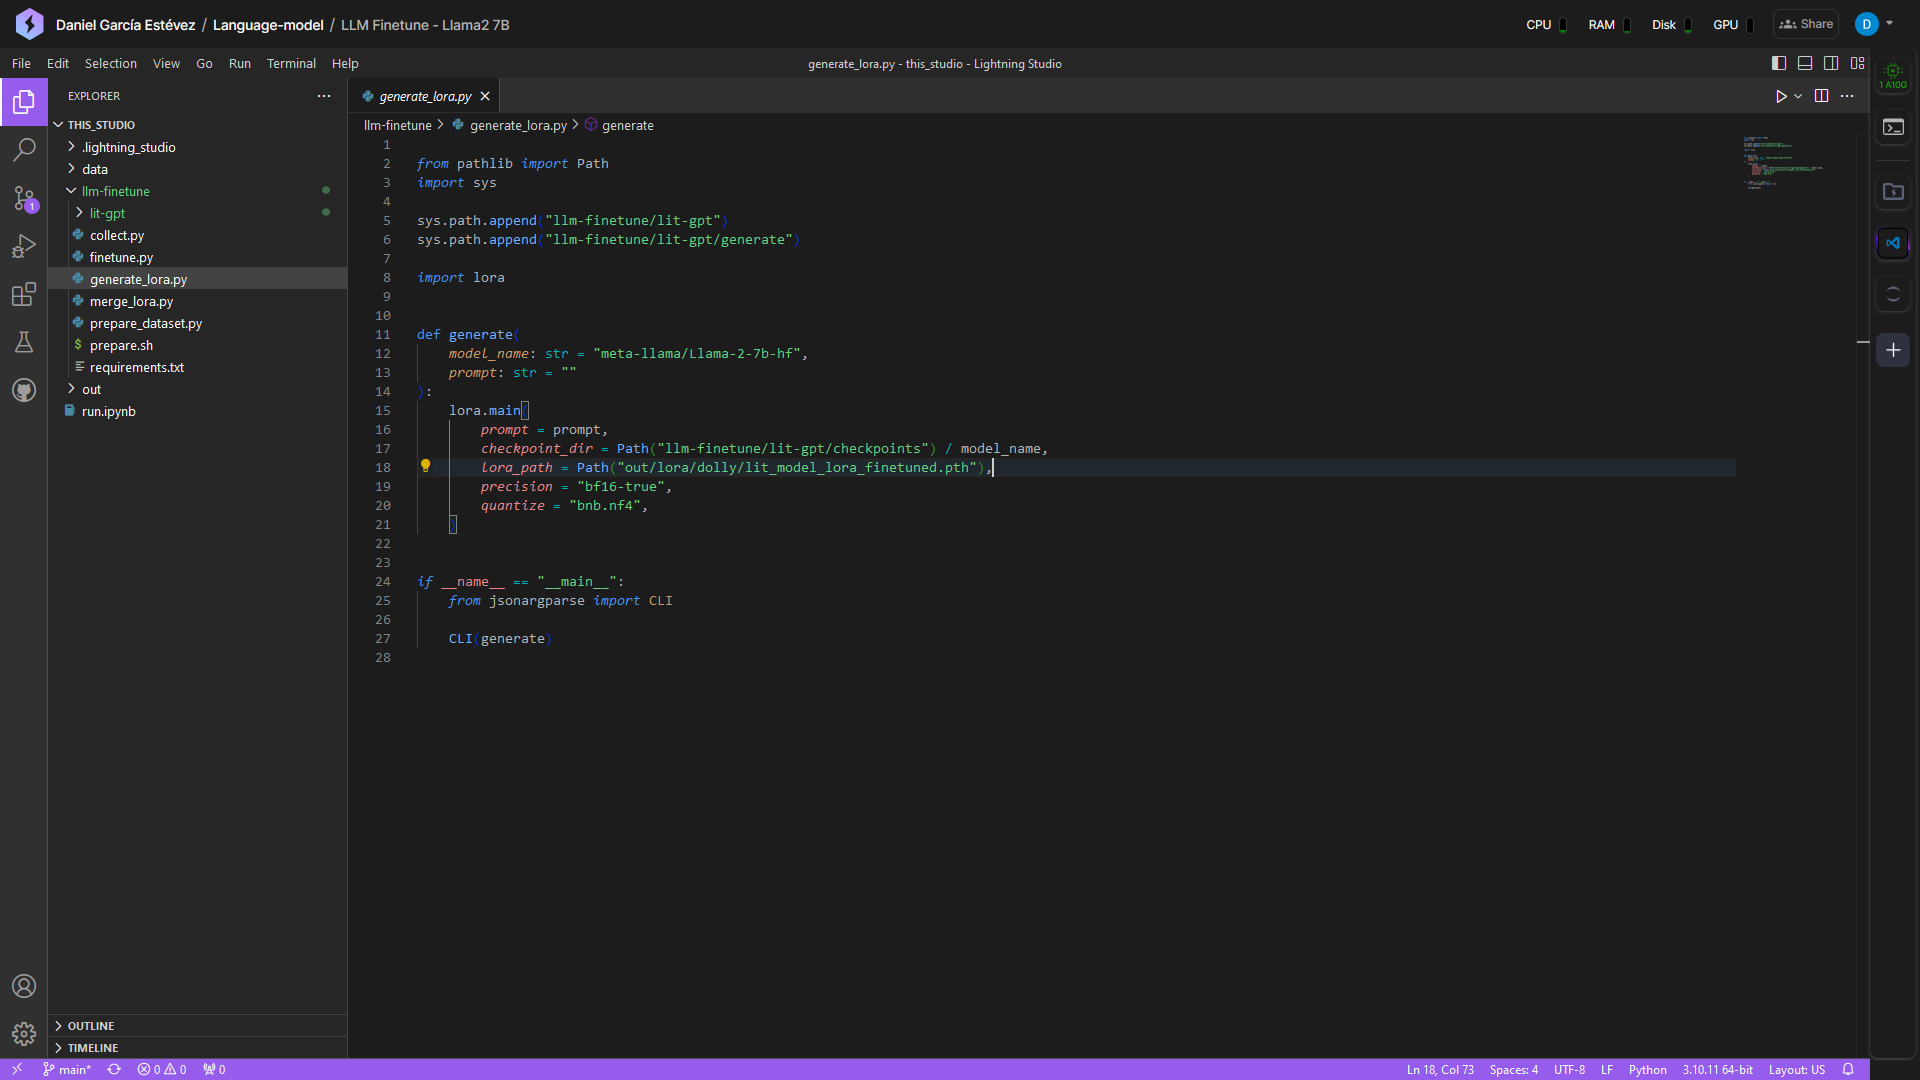
\includegraphics[scale=0.3]{figuras/Capitulo_08/Lightning_Studio.png}
    \end{center}
    \caption[Captura de pantalla de la interfaz de usuario de Lightning Studio]{Captura de pantalla de la interfaz de usuario de Lightning Studio (Elaboración propia)}
    \label{fig:lightning_ia_studio}
\end{figure}

Así mismo, nos ofrece un entorno amigable y sencillo, donde por ejemplo podemos cambiar de
un entorno de CPU a un entorno de GPU y viceversa con un sencillo clic. Nos ofrece estos dos
entornos con las siguientes características:

\begin{itemize}
    \item \textbf{Entorno CPU}
    \begin{itemize}
        \item Un entorno con 4 núcleos de CPU pensado para tareas menos pesadas.
        \item Un entorno con 32 núcleos de CPU pensado para tareas más pesadas como la preparación de conjuntos de entrenamientos muy grandes.
    \end{itemize}
    \item \textbf{Entorno GPU: }
    \begin{itemize}
        \item 1 o 4 NVIDIA A10 Tensor core optimizada para trabajos de IA
        \item 1 o 4 NVIDIA V100 Tensor core optimizada para trabajos de IA
        \item 1 o 4 NVIDIA T4 Tensor core optimizada para trabajos de IA
    \end{itemize}
\end{itemize}

El servicio de Lightning IA Studio sigue un modelo de pago por uso. Donde se utilizan
créditos que equivalen a horas de GPU. Concretamente, 15 créditos nos da para 6 horas de
uso en la GPU. Así mismo, nos ofrecen 15 créditos gratuitos cada mes. \cite{lightningiaPricing}

\subsubsection{Limitaciones}
\label{subsubsec:limitaciones}

% Corregido 08/01/2024
% TODO:daniel: Revisar limitaciones de Lightning IA Studio

La principal limitación que tiene esta plataforma es que es un servicio de pago que dentro
del contexto de este proyecto no se ha asumido debido a que se ha utilizado como refuerzo, es
decir, donde no se ha llegado con el clúster del departamento de Arquitectura de Computadores
se ha llegado con esta solución.

\section{Ejecución}
\label{sec:ejecucion}

En ambos entornos se ha ejecutado el mismo conjunto de entrenamiento. Este conjunto de
entrenamiento se ha generado con el sistema de scripts que se ha desarrollado en el capítulo
\ref{cap:diseñoImplentacion_scripts}.

\subsection{Creación del conjunto de entrenamiento}
\label{subsec:creacion_conjunto_entrenamiento}

\subsubsection{Estrategia 1}
\label{subsubsec:creacion_conjunto:estrategia_1}

En el código \ref{code:DataSet_Estrategia_1} tenemos el conjunto de comandos que se han
utilizado para generar el conjunto de entrenamiento para la estrategia 1. En este conjunto
de comandos se ha utilizado el script \textit{main.py} que se ha desarrollado en el capítulo
\ref{cap:diseñoImplentacion_scripts}. Este script nos permite clonar los repositorios de
los proyectos, compilarlos y generar el conjunto de entrenamiento. Así mismo, se ha copiado
el conjunto de entrenamiento a la carpeta \textit{data} del proyecto de \textit{lit-gpt}.
Por último, se ha copiado el script de preparación de la estrategia 1 a la carpeta \textit{scripts}
del proyecto de \textit{lit-gpt}.

\begin{mycode}
    \begin{minted}{bash}
# Clonamos los repositorios y compilamos
$HOME/soft/bin/python ./src/main.py -r -c ./data/compiler/compilerOptions.json

# Generamos el conjunto de entrenamiento
$HOME/soft/bin/python ./src/main.py -D -d

# Copiamos el conjunto de entrenamiento
mkdir data/Estrategia_1
cp \
/scratch/nas/3/danielg/TFG-Development/output/dataset/dataSet.json 
/scratch/nas/3/danielg/lit-gpt/data/Estrategia_1/dataSet.json

# Copiamos el script de preparación
cp scripts/prepare_alpaca.py scripts/prepare_Estrategia_1.py
    \end{minted}
    \caption[Comando para generar el conjunto de entrenamiento para la estrategia 1]{Comando para generar el conjunto de entrenamiento para la estrategia 1 (Elaboración propia)}
    \label{code:DataSet_Estrategia_1}
\end{mycode}

\subsubsection{Estrategia 2}
\label{subsubsec:creacion_conjunto:estrategia_2}

En el código \ref{code:DataSet_Estrategia_2} tenemos el conjunto de comandos que se han
utilizado para generar el conjunto de entrenamiento para la estrategia 2. En este conjunto
de comandos se ha utilizado el script \textit{prepare-train-data.py} que podemos encontrar
en el repositorio de \textit{neural-compilers}. Este script nos permite generar un conjunto
de entrenamiento con una secuencia de tokens baja. Así mismo, se ha copiado el conjunto
de entrenamiento a la carpeta \textit{data} del proyecto de \textit{lit-gpt}. Por último,
se ha copiado el script de preparación de la estrategia 2 a la carpeta \textit{scripts}
del proyecto de \textit{lit-gpt}.

\begin{mycode}
    \begin{minted}{bash}
# Clonamos el repositorio de neural-compilers
git clone https://github.com/jordiae/neural-compilers.git
cd neural-compilers

# Instalamos dependencias
bash setup.sh

# Generamos el conjunto de entrenamiento
python prepare-train-data.py --config-file configs/data_configs/data-config1.json

# Copiamos el conjunto de entrenamiento
mkdir data/Estrategia_2
cp \
/scratch/nas/3/danielg/TFG-Development/ data/dataset/Estrategia_2.json 
/scratch/nas/3/danielg/lit-gpt/data/Estrategia_2/dataSet.json

# Copiamos el script de preparación
cp scripts/prepare_alpaca.py scripts/prepare_Estrategia_2.py
    \end{minted}
    \caption[Comando para generar el conjunto de entrenamiento para la estrategia 2]{Comando para generar el conjunto de entrenamiento para la estrategia 2 (Elaboración propia)}
    \label{code:DataSet_Estrategia_2}
\end{mycode}

\subsection{Cluster AC: \textit{Sert}}
\label{subsec:cluster_ac_ejecucion}

\subsubsection{Estrategia 1}
\label{subsubsec:cluster_ac_ejecucion:estrategia_1}

En el entorno del cluster AC se ha ejecutado la estrategia 1 y la estrategia 2. Para la
ejecución de la estrategia 1 se ha utilizado los siguientes comandos que se pueden encontrar
en el código \ref{code:Ejecución_Estrategia_1}.

\begin{mycode}
    \begin{minted}{bash}
$HOME/soft/bin/python scripts/prepare_Estrategia_1.py --destination_path data/Estrategia_1/ --max_seq_length 2048

$HOME/soft/bin/python finetune/lora.py --data_dir data/Estrategia_1 --checkpoint_dir checkpoints/stabilityai/stablecode-completion-alpha-3b --out_dir out/lora/Estrategia_1 --precision 16-true --quantize bnb.nf4
    \end{minted}
    \caption[Comandos para ejecutar el \textit{finetuning} con la estrategia 1]{Comandos para ejecutar el \textit{finetuning} con la estrategia 1 (Elaboración propia)}
    \label{code:Ejecución_Estrategia_1}
\end{mycode}

Una vez ejecutado estos comandos se han obenido las siguientes metricas de entrenamiento:

\begin{itemize}
    \item 
\end{itemize}

\subsubsection{Estrategia 2}
\label{subsubsec:cluster_ac_ejecucion:estrategia_2}

Para la ejecución de la estrategia 2 se ha utilizado los siguientes comandos que se
pueden encontrar en el código \ref{code:Ejecución_Estrategia_2}.

\begin{mycode}
    \begin{minted}{bash}
$HOME/soft/bin/python scripts/prepare_Estrategia_2.py --destination_path data/Estrategia_2/ --max_seq_length 2048

$HOME/soft/bin/python finetune/lora.py --data_dir data/Estrategia_2 --checkpoint_dir checkpoints/stabilityai/stablecode-completion-alpha-3b --out_dir out/lora/Estrategia_2 --precision 16-true --quantize bnb.nf4
\end{minted}
    \caption[Comandos para ejecutar el \textit{finetuning} con la estrategia 2]{Comandos para ejecutar el \textit{finetuning} con la estrategia 2 (Elaboración propia)}
    \label{code:Ejecución_Estrategia_2}
\end{mycode}

Una vez ejecutado estos comandos se han obenido las siguientes metricas de entrenamiento:

\begin{itemize}
    \item 
\end{itemize}

\subsection{Lightning IA Studio}
\label{subsec:lightning_ia_studio_ejecucion}

En el entorno de Lightning IA Studio se ha ejecutado tan solo la estrategia 2, ya que
esta es la que a nivel de recursos computacionales es más exigente. Para la ejecución
de la estrategia 2 se ha utilizado los mismos pasos que se han utilizado en el cluster
del departamento de Arquitectura de Computadores que se explica en el código \ref{code:Ejecución_Estrategia_2}.



